
\section{Derivations and numerical example}
\label{app:olg_proofs}

The log specification gives closed-form household policies on the branches
used in the text.  This appendix collects the derivations and describes the
numerical transition.

\subsection{Old-age problems}
\label{app:olg_old_households}

An old renter with financial wealth $a$ solves
\begin{align}
 V_t^R(a)=\max_{c^2,h^2,e}\;&
 \log c^2+\gamma\log h^2+\omega_B\log e \\
 \text{s.t.}\quad&c^2+qe+q\,r_th^2=a+T_t,\qquad
 0<h^2\leq h_R^{\max}.\nonumber
 \label{eq:olg_app_old_renter}
\end{align}
For an old owner, define
\begin{equation}
 A=1+\gamma+\omega_B,\qquad
 \varrho_t=q\,r_t-\ell_t,\qquad
 X_t=a+(P_t-\ell_t)H+T_t.
 \label{eq:olg_app_old_objects}
\end{equation}
The owner problem is \eqref{eq:olg_old_owner}.  Both old problems are strictly
concave on their feasible sets.

\begin{lemma}[Old-age allocations]
\label{lem:olg_old_allocations}
Suppose $r_t>0$, $\varrho_t>0$, and resources place the household in the log
domain.  If the renter size limit is slack, then
\begin{equation}
 c^2=\frac{a+T_t}{A},\qquad
 h^2=\frac{\gamma(a+T_t)}{Aq\,r_t},\qquad
 e=\frac{\omega_B(a+T_t)}{Aq}.
 \label{eq:olg_app_old_renter_interior}
\end{equation}
If the renter limit binds, set $Z^R=a+T_t-q\,r_t h_R^{\max}$; then
\begin{equation}
 h^2=h_R^{\max},\qquad
 c^2=\frac{Z^R}{1+\omega_B},\qquad
 e=\frac{\omega_BZ^R}{(1+\omega_B)q}.
 \label{eq:olg_app_old_renter_cap}
\end{equation}
If both owner constraints are slack, then
\begin{equation}
 c^2=\frac{X_t}{A},\qquad
 h^2=\frac{\gamma X_t}{A\varrho_t},\qquad
 e=\frac{\omega_BX_t}{Aq},
 \label{eq:olg_app_old_owner_interior}
\end{equation}
and the two strict slackness conditions are
\begin{equation}
 \frac{\gamma X_t}{A\varrho_t}<H,\qquad
 \omega_B\varrho_t>\gamma qP_{t+1}.
 \label{eq:olg_app_old_slackness}
\end{equation}
\end{lemma}

\begin{proof}
The result is an expenditure-share calculation.  Consider first the generic
interior budget $c^2+qe+p_hh^2=X$.  The first-order conditions allocate
spending across consumption, housing, and the estate in the proportions
$1:\gamma:\omega_B$:

\begin{equation*}
 p_hh^2=\gamma c^2,\qquad qe=\omega_Bc^2,
 \qquad Ac^2=X.
\end{equation*}

For a renter, set $p_h=q r_t$; for an owner, set $p_h=\varrho_t$.  This gives
the two interior rows.  If the rental limit binds, housing is fixed and the
remaining resources are divided between consumption and the estate in the
proportions $1:\omega_B$, which gives
\eqref{eq:olg_app_old_renter_cap}.  Finally, substituting the interior owner
policy into $h^2<H$ and $e>P_{t+1}h^2$ gives the two slackness conditions.
\end{proof}

Other owner corners are obtained by fixing $h^2=H$, $e=P_{t+1}h^2$, or both,
and allocating the residual resources across the unconstrained uses.  Strict
concavity makes each branch unique.

In the interior owner region, the indirect value and relevant envelopes are
\begin{align}
 V_t^O(a,H)
 &=A\log X_t-A\log A+\gamma\log\gamma-\gamma\log\varrho_t
   +\omega_B\log\omega_B-\omega_B\log q,
 \label{eq:olg_app_old_indirect}\\
 V_{a,t}^O&=\frac{A}{X_t}=\frac1{c_t^2},\qquad
 V_{H,t}^O=(P_t-\ell_t)V_{a,t}^O.
 \label{eq:olg_app_old_envelopes}
\end{align}

\subsection{Young household solutions and tenure}
\label{app:olg_young_households}

The renter and owner problems are those in the main text.  Let
$\lambda_t^m$ be the current-budget multiplier, $\eta_t^m$ the multiplier on
the tenure-specific housing limit, $\upsilon_t^m$ the multiplier on $a'\geq0$,
and $\mu_t$ the owner down-payment multiplier.  Using
$x_t^m=c_t^m-\chi n_t^m$ and $s_t^m=h_t^m-\kappa n_t^m$, the common
consumption and fertility conditions are
\begin{align}
 \lambda_t^m&=\frac1{x_t^m},
 \label{eq:olg_app_young_lambda}\\
 \frac{\vartheta_t}{n_t^m}
 &=\frac{\chi}{x_t^m}+\frac{\alpha\kappa}{s_t^m}.
 \label{eq:olg_app_young_fertility_kkt}
\end{align}
The saving conditions are
\begin{align}
 \lambda_t^R&=\beta R_f V_{a,t+1}^R+\upsilon_t^R,\\
 \lambda_t^O&=\beta R_f V_{a,t+1}^O+\upsilon_t^O,
 \qquad \upsilon_t^ma_t^{\prime m}=0.
 \label{eq:olg_app_saving_kkt}
\end{align}

The main text presents the interior old-age branch.  To include the case in
which an old renter is constrained at $h_R^{\max}$, define
\begin{equation}
 (k_{t+1}^m,\widetilde w_{it}^m)=
 \begin{cases}
 (\beta A,w_{it}),&\text{if old-age choices are interior},\\
 (\beta(1+\omega_B),w_{it}-q^2\,r_{t+1}h_R^{\max}),
 &\text{if $m=R$ and the old rental limit binds}.
 \end{cases}
 \label{eq:olg_old_branch_objects}
\end{equation}
Here $k_{t+1}^m$ is the saving load implied by the Euler equation and
$\widetilde w_{it}^m$ is lifetime wealth net of any committed old-age rent.
On either branch, the young household's reduced lifetime problem, up to a
constant, is
\begin{align}
 \max_{x,s,n}\quad &(1+k_{t+1}^m)\log x+\alpha\log s+
 \vartheta_t\log n \nonumber\\
 \text{s.t.}\quad &(1+k_{t+1}^m)x+u_t^m s+
 (\chi+\kappa u_t^m)n=\widetilde w_{it}^m.
 \label{eq:olg_lifetime_problem}
\end{align}
Equivalently, its budget in gross housing is
\begin{equation}
 (1+k_{t+1}^m)x+\chi n+u_t^mh=\widetilde w_{it}^m.
 \label{eq:olg_lifetime_budget}
\end{equation}

For a renter on either old-age branch in
\eqref{eq:olg_old_branch_objects}, and for an owner whose next-period retention
and estate-composition constraints are slack, the housing conditions reduce to
\begin{equation}
 \frac{\alpha x_t^m}{s_t^m}
 =u_t^m+\zeta_t^m,\qquad
 \zeta_t^R=\frac{\eta_t^R}{\lambda_t^R},\qquad
 \zeta_t^O=
 \frac{\mu_t}{\lambda_t^O}(1-\phi)P_t
 +\frac{\eta_t^O}{\lambda_t^O}.
 \label{eq:olg_app_housing_kkt}
\end{equation}
This proves \eqref{eq:olg_access_wedge}.  If the owner-size limit is slack,
the second term in $\zeta_t^O$ is zero and the access wedge is purely financial.

Writing $B_{it}^m=1+k_{t+1}^m+\alpha+\vartheta_t$, an unconstrained household
chooses
\begin{equation}
 x_t^m=\frac{\widetilde w_{it}^m}{B_{it}^m},\qquad
 s_t^m=\frac{\alpha\widetilde w_{it}^m}{B_{it}^m u_t^m},\qquad
 n_t^m=\frac{\vartheta_t\widetilde w_{it}^m}
 {B_{it}^m(\chi+\kappa u_t^m)}.
 \label{eq:olg_unconstrained_policies}
\end{equation}
Gross choices are $c_t^m=x_t^m+\chi n_t^m$ and
$h_t^m=s_t^m+\kappa n_t^m$.
If the current housing limit binds, substituting
$h_t^m=\widehat h_{it}^m$ into the budget and fertility condition leaves the
single equation
\begin{equation}
 \frac{\vartheta_t}{n}
 -\frac{\alpha\kappa}{\widehat h_{it}^m-\kappa n}
 -\frac{(1+k_{t+1}^m)\chi}
 {\widetilde w_{it}^m-u_t^m\widehat h_{it}^m-\chi n}=0.
 \label{eq:olg_binding_fertility}
\end{equation}
This is the substituted version of the two transparent conditions
\eqref{eq:olg_binding_budget}--\eqref{eq:olg_binding_fertility_foc} in the main
text.

Eliminating old-age choices turns both tenure problems into the same static
allocation problem.  They differ only in user cost, effective wealth, and the
housing limit.

\begin{proposition}[Lifetime reduction and conditional policies]
\label{prop:olg_app_conditional_policies}
Suppose young saving is interior.  For owners, suppose next-period old
retention and estate composition are interior.  For renters, allow either an
interior old housing choice or a strictly binding old rental limit.  Then the
branch objects in \eqref{eq:olg_old_branch_objects} give the lifetime budget
\eqref{eq:olg_lifetime_budget}.  If the current housing limit is slack, the
policies are \eqref{eq:olg_unconstrained_policies}.  Saving on the interior
old-renter, capped old-renter, and interior old-owner branches is, respectively,
\begin{align}
 a_t^{\prime R,I}&=\beta A x_t^R-qT_{t+1},
 \label{eq:olg_app_renter_saving}\\
 a_t^{\prime R,C}&=\beta(1+\omega_B)x_t^R-qT_{t+1}
 +q^2\,r_{t+1}h_R^{\max},
 \label{eq:olg_app_renter_capped_saving}\\
 a_t^{\prime O}&=\beta A x_t^O-qT_{t+1}
 -[q(P_{t+1}-\ell_{t+1})-\phi P_t]h_t^O.
 \label{eq:olg_app_owner_saving}
\end{align}
The capped renter row applies when its implied old allocation satisfies
$\gamma c_{t+1}^2/h_R^{\max}>q\,r_{t+1}$; the interior row applies with the
reverse strict inequality.  Equality is the boundary between the two rows.
If the effective housing limit binds, $h_t^m=\widehat h_{it}^m$ and fertility
is the unique root of \eqref{eq:olg_binding_fertility} in
\begin{equation}
 0<n<\min\left\{
 \frac{\widehat h_{it}^m}{\kappa},
 \frac{\widetilde w_{it}^m-u_t^m\widehat h_{it}^m}{\chi}
 \right\}.
 \label{eq:olg_app_binding_domain}
\end{equation}
\end{proposition}

\begin{proof}
On every stated branch, the old household's marginal value of wealth is
$V_{a,t+1}=1/c_{t+1}^2$.  The saving Euler equation therefore gives
$c_{t+1}^2=\beta R_fx_t$.  For an owner, total old-age resources are
\begin{equation}
 X_{t+1}=R_fa_t'-R_f\phi P_th_t
 +(P_{t+1}-\ell_{t+1})h_t+T_{t+1}.
 \label{eq:olg_app_owner_old_resources}
\end{equation}
Interior old-age expenditure shares give $qX_{t+1}=\beta A x_t$.  Combining
this identity with the current owner budget cancels the mortgage inflow against
its repayment and leaves
$(1+\beta A)x_t+\chi n_t+u_t^Oh_t=w_{it}$.

For an interior old renter, $X_{t+1}=R_fa_t'+T_{t+1}$ and the same argument gives
$a_t'=\beta A x_t-qT_{t+1}$.  If the old rental limit binds, instead define
\begin{equation}
 Z_{t+1}^R=R_fa_t'+T_{t+1}-q\,r_{t+1}h_R^{\max}.
 \label{eq:olg_app_capped_renter_resources}
\end{equation}
Equation~\eqref{eq:olg_app_old_renter_cap} gives
$c_{t+1}^2=Z_{t+1}^R/(1+\omega_B)$, so the Euler equation implies
$qZ_{t+1}^R=\beta(1+\omega_B)x_t$.  Combining this identity with the young
budget gives the second row of \eqref{eq:olg_old_branch_objects}, the capped
saving rule \eqref{eq:olg_app_renter_capped_saving}, and
\eqref{eq:olg_lifetime_budget}.  Thus the committed old-age rent changes both
the consumption weight and effective lifetime resources.

When housing is unconstrained,
\eqref{eq:olg_app_housing_kkt} gives $s=\alpha x/u_t^m$ and
\eqref{eq:olg_app_young_fertility_kkt} gives
$n=\vartheta_t x/(\chi+\kappa u_t^m)$.  Substitution into the lifetime budget
gives $\widetilde w_{it}^m=(1+k_{t+1}^m+\alpha+\vartheta_t)x$, proving
\eqref{eq:olg_unconstrained_policies}.

When the limit binds, substitute $h=\widehat h$ and
$x=(\widetilde w^m-u_t^m\widehat h-\chi n)/(1+k_{t+1}^m)$ into the fertility condition.
This gives \eqref{eq:olg_binding_fertility}.  Its left side tends to $+\infty$
at the lower boundary of \eqref{eq:olg_app_binding_domain} and to $-\infty$
at the upper boundary.  It is strictly decreasing because its derivative is
\begin{equation}
 -\frac{\vartheta_t}{n^2}
 -\frac{\alpha\kappa^2}{(\widehat h-\kappa n)^2}
 -\frac{(1+k_{t+1}^m)\chi^2}
 {(\widetilde w^m-u_t^m\widehat h-\chi n)^2}<0.
\end{equation}
The binding branch therefore has exactly one interior fertility choice.
\end{proof}

At a zero-saving or different old-age corner, the corresponding KKT system
replaces the closed-form policy above.  Strict concavity still gives a unique
conditional tenure choice.

With the logistic ownership preference in \eqref{eq:olg_owner_share}, the
conditional probability of ownership is strictly between zero and one whenever
the two conditional values are finite.  Because the owner-share formula and
the conditional policies are continuous, aggregate choices are continuous
across the rent--own indifference locus.  Other atomless continuous preference
distributions give the same regularity, although not generally the same
closed-form share.

\subsection{Aggregation and positive steady states}
\label{app:olg_steady_states}

Let $F$ denote the distribution of observed young types $i=(y_i,b_i)$.  The
old-state distribution is over financial wealth $a$, inherited owner housing
$H$, and tenure.  For any bounded measurable test function $\psi$, its law of
motion is
\begin{align}
 \int\psi\,\dd G_{t+1}
 =\int\Big[&(1-\pi_t^O(i))
 \psi(R_fa_t^{\prime R}(i),0,R)\nonumber\\[-2pt]
 &+\pi_t^O(i)\psi(R_fa_t^{\prime O}(i)-R_f\phi P_th_t^O(i),h_t^O(i),O)
 \Big]\,\dd F(i).
 \label{eq:olg_app_distribution_law}
\end{align}
Average fertility and young housing integrate the corresponding conditional
policies with the same weights.  Average old housing integrates the old
policies over $G_t$.  Average taxable sales are
\begin{equation}
 \bar h_t^{\mathrm{sell}}=\int\mathbf 1\{m=O\}
 [H-h_t^2(a,H,O)]\,\dd G_t.
 \label{eq:olg_app_old_sales}
\end{equation}
Equations \eqref{eq:olg_housing_clearing}--\eqref{eq:olg_government}, the cohort
laws, and \eqref{eq:olg_app_distribution_law} close the economy.

\begin{proof}[Proof of Proposition~\ref{prop:olg_steady_state}]
The cohort laws do most of the work.  Since today's old are yesterday's young,
$O^*=Y^*$.  A constant young cohort then requires
$1=\nu\bar n(P^*,T^*;\vartheta)$: average fertility must be at replacement.
A constant real house price makes taxable gains zero.  Housing clearing sets
the common cohort mass at $Y^*=\bar H/\bar h$.  Finally, the government budget
is $2Y^*T^*=q\tau^pP^*\bar H$; substituting for $Y^*$ gives the transfer
equation in \eqref{eq:olg_steady_state_system}.  Reversing these steps proves
sufficiency once the stationary household distribution is constructed.
\end{proof}

Existence can be shown in two one-dimensional steps.  For each candidate house
price, the fiscal rule determines a transfer.  Moving along this fiscal locus,
a steady state is a price at which fertility equals replacement.  The
following proposition makes that argument precise and also makes clear that a
positive steady state is not guaranteed for arbitrary primitives.

\begin{proposition}[Steady-state existence and local uniqueness]
\label{prop:olg_app_ss_existence}
Let
$\mathcal D=[\underline P,\overline P]\times
[\underline T,\overline T]\subset\mathbb R_{++}^2$ be a rectangle on which
conditional policies are feasible, relevant user costs are positive, and
$\bar n$ and $\bar h$ are continuous.  For the local-uniqueness statement,
suppose they are continuously differentiable near the steady state.  Define
\begin{equation}
 \Psi(P,T)=\frac{q\tau^pP}{2}\bar h(P,T;\vartheta).
 \label{eq:olg_app_fiscal_map}
\end{equation}
Suppose:
\begin{enumerate}
 \item $\Psi(P,\cdot)$ maps
 $[\underline T,\overline T]$ into itself for every $P$, and there is an
 $L<1$ such that $|\Psi(P,T)-\Psi(P,T')|\leq L|T-T'|$ for all
 $P\in[\underline P,\overline P]$ and
 $T,T'\in[\underline T,\overline T]$;
 \item writing $T=\mathcal T(P)$ for its unique fixed point,
 \begin{equation}
 [\nu\bar n(\underline P,\mathcal T(\underline P);\vartheta)-1]
 [\nu\bar n(\overline P,\mathcal T(\overline P);\vartheta)-1]<0.
 \label{eq:olg_app_replacement_boundary}
 \end{equation}
\end{enumerate}
Then a positive steady state exists in $\mathcal D$.  It is locally unique if
\begin{equation}
 J^*=\begin{bmatrix}
 \nu\bar n_P & \nu\bar n_T\\[2pt]
 -\dfrac{q\tau^p}{2}(\bar h+P\bar h_P)&
 1-\dfrac{q\tau^pP}{2}\bar h_T
 \end{bmatrix}_{(P^*,T^*;\vartheta)}
 \label{eq:olg_app_ss_jacobian}
\end{equation}
is nonsingular.
\end{proposition}

\begin{proof}
Fix a price $P$.  The contraction theorem gives a unique transfer
$\mathcal T(P)$ that balances the government budget.  Uniform contraction and
continuity of the fiscal map make this transfer continuous in $P$.  The
replacement residual therefore varies continuously along the fiscal locus.
The boundary sign change and the intermediate value theorem produce a price
$P^*$ at which fertility is exactly $1/\nu$.  Its fiscal fixed point
$T^*=\mathcal T(P^*)$ completes the steady state.  If $J^*$ is nonsingular,
the implicit-function theorem gives local uniqueness.
\end{proof}

The first condition can be checked from bounds on primitives and policies.  For
example, suppose $0<\underline h\leq\bar h\leq\overline h$ on
$\mathcal D$ and $\bar h(P,\cdot)$ is uniformly Lipschitz with constant
$L_h$.  It is enough to choose transfer bounds such that
\begin{equation}
 \underline T\leq\frac{q\tau^p\underline P}{2}
 \underline h,\qquad
 \overline T\geq\frac{q\tau^p\overline P}{2}
 \overline h,
 \qquad
 \frac{q\tau^p\overline P}{2}L_h<1.
 \label{eq:olg_app_fiscal_primitive_bounds}
\end{equation}
The replacement boundary condition requires average fertility to lie on
opposite sides of $1/\nu$ at the two price bounds, after closing the fiscal
account.  It can be checked directly from the household policies.

If $J^*$ is nonsingular, the response to a permanent change in $\vartheta$ is
\begin{equation}
 \begin{bmatrix}P_\vartheta^*\\T_\vartheta^*\end{bmatrix}
 =-(J^*)^{-1}
 \begin{bmatrix}
 \nu\bar n_\vartheta\\[2pt]
 -\dfrac{q\tau^pP^*}{2}\bar h_\vartheta
 \end{bmatrix}.
 \label{eq:olg_app_ss_comparative_static}
\end{equation}
The associated population-scale response is
\begin{equation}
 \frac{\dd\log Y^*}{\dd\vartheta}
 =-\frac{\bar h_PP_\vartheta^*+
 \bar h_TT_\vartheta^*+\bar h_\vartheta}{\bar h}.
 \label{eq:olg_app_scale_response}
\end{equation}
There is no general sign without restrictions on the demand and tenure
elasticities.

\subsection{Transition equilibrium}
\label{app:olg_transitions}

Suppose $\vartheta_t=\vartheta^0$ for $t<0$ and
$\vartheta_t=\vartheta^1$ for $t\geq0$, and both values support regular positive
steady states $\mathcal E^0$ and $\mathcal E^1$.  The date-zero state is the old
steady state: $S_0=(Y^0,Y^0,G^0,P^0)$.  In particular, $P_{-1}=P^0$ is the
basis of date-zero old owners.  No additional initialization shock is present.

The gains rule is equivalently the complementarity system
\begin{equation}
 \ell_t\geq0,\qquad
 \ell_t\geq\tau^g(P_t-P_{t-1}),\qquad
 \ell_t[\ell_t-\tau^g(P_t-P_{t-1})]=0.
 \label{eq:olg_app_gains_complementarity}
\end{equation}
It is continuous but kinked.  Within an appreciating regime its price
derivative is $\tau^g$; within a non-appreciating regime it is zero.

Fix a terminal date $J$ and set prices and transfers from $J+1$ onward equal to
their new steady-state values.  A household that buys at $J$ nevertheless
keeps $P_J$ as its tax basis, so its old-age gains tax is computed correctly.
The state generated at $J+1$ is recorded rather than set equal to its
steady-state value.  Let $z_J$ stack
$(\log P_0,\ldots,\log P_J,\log T_0,\ldots,\log T_J)$ and order the residuals
as the $J+1$ housing equations followed by the $J+1$ government equations.
Recursively applying household policies, the distribution
law, and cohort laws turns \eqref{eq:olg_transition_residuals} into a finite
system
\begin{equation}
 \mathbf R_J(z_J;\varepsilon)=0,
 \label{eq:olg_app_stacked_transition}
\end{equation}
where $\varepsilon$ scales the permanent change from $\vartheta^0$ to
$\vartheta^1$ and the terminal steady state also varies with $\varepsilon$.

The gains rule has a kink at constant prices.  To handle it, fix a candidate
appreciation pattern
$d=(d_0,\ldots,d_{J+1})\in\{0,1\}^{J+2}$ and define the smooth branch
\begin{equation}
 \ell_t^d=\tau^g d_t(P_t-P_{t-1}).
 \label{eq:olg_app_gains_branch}
\end{equation}
It agrees with the statutory rule when prices rise on dates with $d_t=1$ and
fall on dates with $d_t=0$.  Let $\mathbf R_J^d$ denote the residual system on
this branch.

\begin{proposition}[Local solution for a fixed terminal date]
\label{prop:olg_app_local_transition}
Suppose the old steady state is regular, the household active sets are strict,
and the Jacobian $\partial\mathbf R_J^d/\partial z_J$ is nonsingular at the old
steady state.  If the directional response of $P_t-P_{t-1}$ is positive on
dates with $d_t=1$ and negative on dates with $d_t=0$, then, for each fixed
$J$, a sufficiently small positive shock has a locally unique terminally
closed solution on branch $d$.  This solution satisfies the statutory gains
rule through date $J+1$.
\end{proposition}

\begin{proof}
On a fixed branch, household policies and equilibrium residuals are smooth.
At zero shock the constant old-steady-state path solves
$\mathbf R_J^d=0$.  The implicit-function theorem therefore gives a locally
unique solution for a small shock.  The assumed price signs persist locally,
so \eqref{eq:olg_app_gains_branch} coincides with the positive-part tax rule.
\end{proof}

The result is silent if a price response is tangent to the kink, and it does
not rule out a solution on another branch.  It is also a result for a fixed
terminal date, not an existence theorem for the infinite-horizon transition.
The horizon comparisons below show that the computed path is insensitive to
extending $J$.

The reason one shock can affect several successive capital-gains bases is the
demographic state.  The initial fertility response changes $Y_1$ through
$Y_1=\nu\bar n_0Y_0$; the resulting young cohort becomes the old cohort one
period later, and subsequent fertility choices continue to update cohort
masses.  With a fixed housing stock, this propagation can move equilibrium
housing demand and prices over several dates.  Whenever a date in that path
has $P_s>P_{s-1}$, the cohort selling at $s$ realizes
$\ell_s=\tau^g(P_s-P_{s-1})$.  In the numerical example, the equilibrium path
determines the sign and duration of appreciation.

\subsection{Compensated reallocation}
\label{app:olg_reallocation}

For a constrained young owner, \eqref{eq:olg_app_housing_kkt} gives the
current-goods marginal value
\begin{equation}
 MV_{it}^Y=\frac{\alpha x_{it}^O}{s_{it}^O}
 =q\,r_t+q\ell_{t+1}+\zeta_{it}^{O,F}.
 \label{eq:olg_app_young_mv}
\end{equation}
For an old incumbent whose retention and estate-composition constraints are
both slack, the housing first-order condition from \eqref{eq:olg_old_owner}
gives
\begin{equation}
 MV_{jt}^O=\frac{\gamma c_{jt}^2}{h_{jt}^2}=q\,r_t-\ell_t.
 \label{eq:olg_app_old_mv}
\end{equation}
Subtracting gives the decomposition in
\eqref{eq:olg_reallocation_surplus}.

To translate the value gap into a welfare comparison, move one marginal unit,
compensate the incumbent, finance the buyer at the market bond price, and
return the incremental tax revenue.  The only resource cost is the cost of
changing title and occupancy.

\begin{assumption}[Implementation]
\label{ass:olg_two_date_ledger}
The marginal transfer can be financed at the bond price, and household-specific
transfers can be made at dates $t$ and $t+1$.  The buyer's old-age retention and
estate constraints are slack.  The added unit is sold at $t+1$ while the
buyer's baseline old-age housing is held fixed.  Fertility, tenure, cohort
masses, and all other allocations are unchanged.
\end{assumption}

\begin{proof}[Proof of Proposition~\ref{prop:olg_reallocation}]
Transfer $\epsilon>0$ units from the old incumbent to the young buyer.  The
baseline has the incumbent retain the unit, transfer it at death with basis
$P_{t+1}$, and have the estate sell it at date $t+1$ without gains tax.  The
following ledger values each change in date-$t$ consumption goods and divides
by $\epsilon$:
\begin{center}
\small
\begin{tabularx}{0.96\textwidth}{@{}lXr@{}}
\toprule
Agent & Change relative to the baseline & Net value\\
\midrule
Incumbent $j$
& Receives $P_t$, pays $\ell_t$, and gives up a unit whose net
service-and-estate value, after property tax, is $P_t-\ell_t$ at the interior
retention choice. & $0$\\
Buyer $i$
& Pays $P_t$ using market-rate bridge finance, pays $q\tau^pP_t$, receives
current services worth $MV_{it}^Y$, and the added unit is sold next period for
$q(P_{t+1}-\ell_{t+1})$. & $\zeta_{it}^{O,F}$\\
Government
& Property-tax revenue is unchanged; the incumbent sale and the buyer's later
sale yield revenue absent from the baseline estate sale. &
$\ell_t+q\ell_{t+1}$\\
Lenders
& Bridge and mortgage funds are supplied at the bond price. & $0$\\
Real resources
& Transferring title and occupancy uses $K_{ijt}$ units of current goods. &
$-K_{ijt}$\\
\midrule
Total && $\zeta_{it}^{O,F}+\ell_t+q\ell_{t+1}-K_{ijt}$\\
\bottomrule
\end{tabularx}
\end{center}
For the buyer row, substituting
$MV_{it}^Y=q\,r_t+q\ell_{t+1}+\zeta_{it}^{O,F}$ and
$q\,r_t=P_t+q\tau^pP_t-qP_{t+1}$ gives the displayed net value.  For the
incumbent row, the retention first-order condition makes the marginal unit's
net service-and-estate value equal to its after-tax sale proceeds:
$MV_{jt}^O-q\tau^pP_t+qP_{t+1}=P_t-\ell_t$.  These identities count the
current housing service and the transfer of title once each.

Assumption~\ref{ass:olg_two_date_ledger} assigns the added unit to the
date-$(t+1)$ sale while holding the buyer's baseline old-age housing fixed.
Slack old-age constraints make this perturbation feasible, and the old-age
first-order conditions make it welfare-neutral to first order.

If total net value is positive, date-$t$ and date-$(t+1)$ transfers can leave
both affected households weakly above baseline and one strictly above it.
Smoothness and the strict first-order inequality imply the same conclusion for
a sufficiently small finite transfer.  At a steady state the two gains terms
are zero, so the condition becomes $\zeta_i^{O,F}>K_{ij}$.
\end{proof}

The Pareto statement depends on the financing and transfers in
Assumption~\ref{ass:olg_two_date_ledger}.  Without them, the value gap remains
a useful decomposition but need not be implementable.  The proposition also
fixes population.  Comparing paths with different populations requires a
social criterion for economies with different people; see
\citet{golosovjonestertilt2007} and \citet{pereznievasetal2019}.

The tax treatment of rental intermediaries affects incidence but not the
decomposition.  If an intermediary also pays $\ell_{t+1}$ upon resale, its
zero-profit rent is $r_t^L=r_t+\ell_{t+1}$.  The young owner's private
current-goods cost becomes $q\,r_t^L$, while the incumbent's retention cost can
be written $q\,r_t^L-\ell_t-q\ell_{t+1}$.  Their difference remains
$\zeta_{it}^{O,F}+\ell_t+q\ell_{t+1}$.

\begin{figure}[H]
\centering
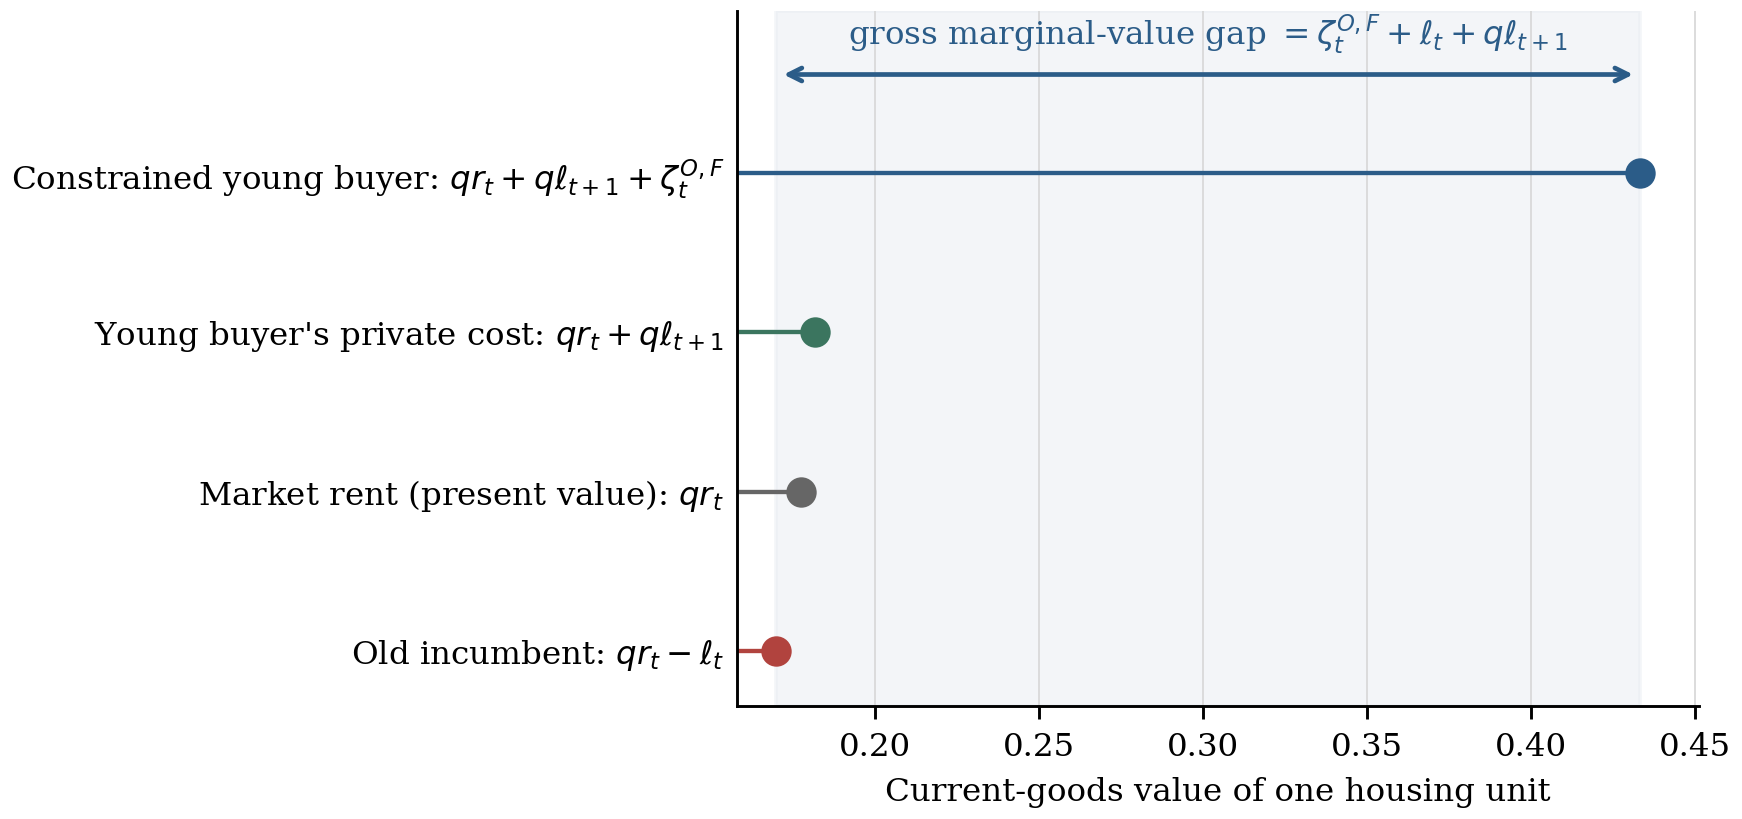
\includegraphics[width=0.88\textwidth]{figures/simplified_olg_reallocation_wedge.png}
\caption{Shadow-value decomposition on the computed path.  The financing wedge
raises the young buyer's value; realization taxes lower the old incumbent's
value and raise the buyer's anticipated private cost.  The displayed object is
the gross marginal-value gap.  Under the ledger in
Proposition~\ref{prop:olg_reallocation}, the reallocation is a Pareto
improvement for current households when this gap exceeds the real transfer
cost.}
\label{fig:olg_reallocation_wedge}
\end{figure}

\subsection{Housing access and fertility}
\label{app:olg_fertility}

Relaxing a binding housing limit has two effects.  It gives the family more
space, which makes children less costly, but it also requires the household to
pay for more housing, which leaves fewer goods for children.  The derivative
below compares these two forces.

Suppose $h=\widehat h$ binds and fertility remains interior.  Define
\begin{equation}
 x=\frac{\widetilde w_{it}^m-u_t^m\widehat h-\chi n}
 {1+k_{t+1}^m},\qquad
 s=\widehat h-\kappa n,
 \label{eq:olg_app_xs_binding}
\end{equation}
and collect the positive terms in
\begin{equation}
 \Delta=\frac{\vartheta_t}{n^2}
 +\frac{\chi^2}{(1+k_{t+1}^m)x^2}
 +\frac{\alpha\kappa^2}{s^2}>0.
 \label{eq:olg_app_fertility_delta}
\end{equation}
Implicit differentiation of the binding-fertility condition gives
\begin{equation}
 \frac{\dd n}{\dd\widehat h}
 =\frac{\alpha\kappa/s^2-\chi u_t^m/
 [(1+k_{t+1}^m)x^2]}{\Delta}.
 \label{eq:olg_fertility_derivative}
\end{equation}
On the interior old-age branch, the derivative is nonnegative exactly when
\begin{equation}
 \chi\leq
 \frac{(1+\beta A)\kappa(u_t^m+\zeta_{it}^m)^2}{\alpha u_t^m}.
 \label{eq:olg_fertility_sign}
\end{equation}

\begin{proof}[Derivation of \eqref{eq:olg_fertility_derivative} and
\eqref{eq:olg_fertility_sign}]
Let the left side of \eqref{eq:olg_binding_fertility} be
$F(n,\widehat h)$.  Direct differentiation gives
\begin{align}
 F_n&=-\Delta<0,\\
 F_{\widehat h}&=\frac{\alpha\kappa}{s^2}
 -\frac{\chi u_t^m}{(1+k_{t+1}^m)x^2}.
\end{align}
The implicit-function theorem gives
$\dd n/\dd\widehat h=-F_{\widehat h}/F_n$, which is
\eqref{eq:olg_fertility_derivative}.  Its numerator is the difference between
the space benefit and the goods-resource cost described above.  At a
constrained allocation,
\eqref{eq:olg_app_housing_kkt} implies
\begin{equation}
 \frac{x}{s}=\frac{u_t^m+\zeta_{it}^m}{\alpha}.
 \label{eq:olg_app_xs_ratio}
\end{equation}
Substituting this ratio into $F_{\widehat h}\geq0$ gives the condition in
\eqref{eq:olg_fertility_sign} on the interior old-age branch, where
$k_{t+1}^m=\beta A$.  On the capped old-renter branch the same derivation uses
$k_{t+1}^R=\beta(1+\omega_B)$.
\end{proof}

The same calculation separates two other partial-equilibrium channels:
\begin{equation}
 \frac{\partial n}{\partial\widetilde w_{it}^m}
 =\frac{\chi}{(1+k_{t+1}^m)x^2\Delta}>0,
 \qquad
 \frac{\partial n}{\partial u_t^m}
 =-\frac{\chi\widehat h}
 {(1+k_{t+1}^m)x^2\Delta}<0.
 \label{eq:olg_app_fertility_wealth_user_cost}
\end{equation}
At a fixed cap, more lifetime resources raise fertility and a higher housing
user cost lowers it.

A primitive sufficient condition, stronger than the exact condition, is
\begin{equation}
 \chi\leq\frac{(1+k_{t+1}^m)\kappa u_t^m}{\alpha},
 \label{eq:olg_app_fertility_sufficient}
\end{equation}
because $\zeta_{it}^m\geq0$.  When the down-payment constraint alone binds,
\begin{equation}
 \widehat h_{it}^O=\frac{b_i}{(1-\phi)P_t},\qquad
 \frac{\partial\widehat h^O}{\partial b_i}
 =\frac1{(1-\phi)P_t},\qquad
 \frac{\partial\widehat h^O}{\partial\phi}
 =\frac{b_i}{(1-\phi)^2P_t}.
 \label{eq:olg_app_cap_pass_through}
\end{equation}
The derivative with respect to $\phi$ isolates the cap-relaxation channel when
prices and resources are held fixed.  The two total derivatives on this branch
are
\begin{align}
 \frac{\partial n}{\partial\phi}
 &=\frac{\partial n}{\partial\widehat h}
 \frac{b_i}{(1-\phi)^2P_t},\\
 \frac{\partial n}{\partial b_i}
 &=\frac{\partial n}{\partial\widetilde w_{it}^O}
 +\frac{\partial n}{\partial\widehat h}
 \frac{1}{(1-\phi)P_t}.
 \label{eq:olg_app_financing_fertility_derivatives}
\end{align}
A change in liquid wealth has both a wealth channel and a housing-access
channel.  A funded policy additionally moves prices, transfers, and tenure,
and its aggregate response requires the equilibrium system.

\subsection{Mixed-tenure example}
\label{app:olg_computation}

The numerical example gives observed types common income and liquid wealth and
retains the logistic ownership preference in \eqref{eq:olg_owner_share}.  It
computes the two steady states and a terminally closed transition between them.
Table~\ref{tab:olg_app_parameters} lists the parameters.

\begin{table}[!htb]
\centering
\caption{Parameters of the mixed-tenure construction}
\label{tab:olg_app_parameters}
\footnotesize
\begin{tabular}{@{}llr@{\qquad}llr@{}}
\toprule
Object & Parameter & Value & Object & Parameter & Value\\
\midrule
Bond price & $q$ & 0.50 & Mortgage share & $\phi$ & 0.80\\
Property tax & $\tau^p$ & 0.05 & Gains-tax rate & $\tau^g$ & 0.20\\
Space weight & $\alpha$ & 0.40 & Space per child & $\kappa$ & 0.50\\
Goods per child & $\chi$ & 0.15 & Young discount & $\beta$ & 0.40\\
Old housing weight & $\gamma$ & 0.30 & Estate weight & $\omega_B$ & 0.40\\
Income & $y$ & 1.00 & Liquid wealth & $b$ & 0.06\\
Household formation & $\nu$ & 2.00 & Housing stock & $\bar H$ & 2.00\\
Rental limit & $h_R^{\max}$ & 0.45 & Owner limit & $h_O^{\max}$ & 2.00\\
Owner intercept & $\bar\xi$ & $-0.15$ & Taste scale & $\sigma_\xi$ & 0.12\\
\bottomrule
\end{tabular}
\end{table}

At date zero, $\vartheta$ rises permanently from $0.35$ to $0.50$.  Solving
\eqref{eq:olg_steady_state_system} gives Table~\ref{tab:olg_app_steady_states}.

\begin{table}[!htb]
\centering
\caption{Positive steady-state endpoints}
\label{tab:olg_app_steady_states}
\footnotesize
\begin{tabular}{@{}lrr@{}}
\toprule
Object & Initial steady state & Final steady state\\
\midrule
Fertility preference $\vartheta$ & 0.3500 & 0.5000\\
Average fertility $\bar n$ & 0.5000 & 0.5000\\
House price $P$ & 0.3427 & 0.4844\\
Per-household transfer $T$ & 0.00589 & 0.00602\\
Young owner share & 0.7486 & 0.5149\\
Renter fertility & 0.3527 & 0.4368\\
Owner fertility & 0.5495 & 0.5596\\
Young renter housing & 0.4500 & 0.4500\\
Young owner housing & 0.8754 & 0.6193\\
Old renter housing & 0.4500 & 0.4500\\
Old owner housing & 0.6582 & 0.4649\\
Young and old cohort mass & 1.4553 & 2.0103\\
\bottomrule
\end{tabular}
\end{table}

Average fertility is $1/\nu=0.5$ at both endpoints, but conditional fertility,
tenure, housing, prices, and population scale differ.  Both roots are locally
regular: the Jacobian determinants in $(\log P,\log T)$ are $-0.00466$ and
$-0.00433$.

On impact, average fertility rises to $0.6223$ and the young cohort expands one
period later.  The price rises from $0.3427$ to $0.3800$, reaches $0.4975$ at
date 3, and then approaches $0.4844$.  Gains taxes are positive on dates 0--3
and 7--8.  Thus one preference change generates taxable gains for several
cohorts even though gains are zero in both steady states.

Both tenures have positive mass.  The young renter and owner housing limits
bind, and the owner's limit is financial.  The old rental limit binds, while
old owners are interior.  The maximum scaled equilibrium residual is
$6.51\times10^{-10}$; extending the horizon from 28 to 32 changes the first
twenty dates by at most $3.11\times10^{-15}$.

The steady-state existence conditions are also satisfied on the declared
price--transfer grid: the fiscal map is a contraction and the replacement
residual changes sign at the two price boundaries.
